38. $f(x)=\cfrac{x+1-|x+1|}{x^2-1}=\begin{cases}\cfrac{2x+2}{(x-1)(x+1)},\ x<-1,\\ 0,\ x>-1,\ x
eq1.\end{cases}=
\begin{cases}\cfrac{2}{x-1},\ x<-1,\\ 0,\ x>-1,\ x
eq1.\end{cases}$
$$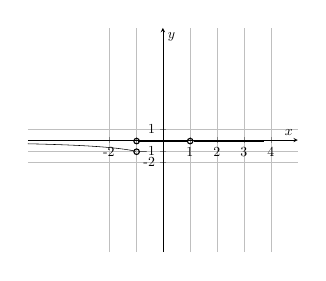
\begin{tikzpicture}[scale=0.5]
\tikzset {line01/.style={line width =0.5pt}}
\tikzset{line02/.style={line width =1pt}}
\tikzset{line03/.style={dashed,line width =0.5pt}}
\begin{axis}[
    axis lines = middle,
    grid=major,
    legend pos={south west},
    xlabel = {$x$},
    %xlabel style={below right},
    ylabel = {$y$},
    xmin=-5,
    xmax=5,
    ymin=-10,
    ymax=10,
    xtick={-2,-1,1, 2,3,4},
    xticklabels={-2,$ $,1, 2,3,4},
    ytick={-2, -1, 1},
    yticklabels={-2, $-1$, 1},
                  ]
	%\addplot[domain=-5:0.99, samples=100, color=black] {0};
    \addplot[domain=-5:-1, samples=100, color=black] {2/(x-1)};
    %\addplot[domain=1.01:5, samples=100, color=black] {2/(x-1)};
    %\addplot[domain=3.01:5, samples=100, color=black] {-1/x};
   % \addplot[domain=1.01:5, samples=100, color=black] {3/(x+1)};
    %\addlegendentry{$\text{Рис. 1}$};
\end{axis}
%\draw (3.8,2.255) circle (2pt);
%\draw (3.8,1.14) circle (2pt);
\draw (2.76,2.82) circle (2pt);
\draw (2.76,2.55) circle (2pt);
\draw (4.12,2.82) circle (2pt);
\draw[line02] (2.8,2.82) -- (4.06,2.82);
\draw[line02] (4.22,2.82) -- (6,2.82);
%\draw[line02] (2.35,1.1) -- (3.75,1.1);
\end{tikzpicture}$$
б) По графику определим $D(f)=(-\infty;-1)\cup(-1;1)\cup(1;+\infty).$\\
в) По графику определим количество решений: $a\in(-\infty;-1]\cup(0;+\infty):0,\ a\in(-1;0): 1,\ a=0:\infty.$\\
